\chapter{绪论}\label{chapter01}
{\em 本章首先介绍研究的立项背景,分析保障系统正确的重要性,并阐述研究意义。其次,综述分析遗忘理论、最强必要(最弱充分)条件等关键技术的国内外研究动态,以及遗忘理论在形式化验证中的应用研究趋势。然后,围绕研究对象凝练出关键问题与目标。进一步,介绍本文的核心研究内容以及研究取得的主要成果。最后,给出具体章节组织安排。}
\section{研究背景与意义}
\subsection{研究背景}

形式化验证是一种广泛应用在硬件\cite{lam2007,lv2000,jani2007Verilog}和软件系统中\cite{yuan2008,gu2005}的有别于测试的、采用数学方法证明系统满足给定特性的验证(verification)技术。软件和硬件的缺陷会导致严重的后果,如表\ref{tab:systemEvents_1.1}中列出的几个重大事件。近年来,为了减少系统(尤其是像火箭发射系统和卫星发射系统等关键领域的系统)错误带来的损失,形式化方法的研究与应用越来越受到人们的重视。包括INTEL、AMD、IBM、NVIDIA、CADENCE、 Motorola、西门子和微软等在内的大型公司纷纷引入了形式化验证方法。与此同时,学术界也在形式化验证领域取得了突破性的成果,比如:剑桥大学进行了ARM6处理器的验证\cite{DBLP:conf/tphol/Fox03},德国的Verisoft项目验证了一个一万行的操作系统内核\cite{DBLP:conf/sefm/DaumSS09}。

\begin{table}[htbp]
\caption{由系统故障引起的重大事件概览}
\label{tab:systemEvents_1.1}
\centering
\fontsize{10pt}{\baselineskip}\selectfont
\begin{tabular}{p{0.12\textwidth}p{0.35\textwidth}p{0.35\textwidth}}%
	\toprule
	\textbf{发生时间}&\textbf{事故事件(系统错误)}&\textbf{造成的损失}\\
	\midrule
    1991年 & 美国爱国者导弹系统舍入错误 & 28名士兵死亡、100人受伤等\\
	1996年 & 阿丽亚娜5型运载火箭因软件不同飞行条件下代码重用 & 导致其与其他卫星在瞬间灰飞烟灭\\
	1999年 & 火星探测器用错度量单位 & 引起探测器坠毁并造成了3.27亿美元的损失\\
	2011年 & 温州7.23动车信号设备在设计上存在严重的缺陷导致 &导致动车脱节脱轨、多人失去生命\\
	
\bottomrule
\end{tabular}
\end{table}

形式化验证有两种主要的验证方法:自动定理证明(Automated theorem proving)和模型检测(Model checking)。
在自动定理证明中,系统模型和规范(specification)被同一形式化语言分别描述为$\varphi_{imp}$和$\varphi_{spec}$,剩下的任务就是证明性质,如:$\varphi_{imp}\rto \varphi_{spec}$或$\varphi_{imp}\lrto\varphi_{spec}$。
常用的自动定理证明方式有基于规约(Resolution)\cite{DBLP:journals/jacm/Robinson65}和常用于模态逻辑的基于表推理(tableau)\cite{hughes1996new}的方法。
然而,在自动定理证明中寻找不变式(invariant)是一个相当困难的问题。
因此,为了避免像Hoare逻辑\cite{Hoare1969}、动态逻辑\cite{harel1979first}和分离逻辑\cite{DBLP:conf/lics/Reynolds02}在形式化验证中寻找不变式,Fangzhen Lin提出将一个程序(program)转换为一阶理论,
然后再使用一阶理论中的自动定理证明方法来验证\cite{DBLP:journals/ai/Lin16}。

形式化验证的模型检测首先由Clarke提出,并用于解决并发系统验证问题\cite{DBLP:conf/spin/Clarke08}。Clarke和Emerson在文章\cite{clarke1981design}中指出,在有限状态的并发系统中使用时态逻辑的推演系统(deductive system)中的公理和推理规则进行构造性证明(proof construction)的方法来证明该系统是否满足给定的规范是不必要的。因为在有限状态并发系统中,该并发系统可以被看作是一个Kripke结构$\Hm$,与此同时,一个规范被表示成一个逻辑公式$\varphi$。此时,该验证问题就变成检验一个Kripke结构是否满足该公式,即模型检测($\Hm\models \varphi$): 判断$\Hm$是否是$\varphi$的一个模型。

近年来,模型检测问题在知识表示与推理(KRR)领域的推进下取得了丰富的科研成果,例如:基于SAT的有界(bounded)模型检测\cite{DBLP:journals/ac/BiereCCSZ03}和基于OBDD的符号模型检测\cite{burch1992symbolic}已经使得模型检测问题在时间和空间效率上取得了很大的进步,在一定程度上缓解了其固有的状态空间爆炸问题。此外,大量优质的模型验证器(如:NuSMV\footnote{http://nusmv.fbk.eu/}、SPIN\footnote{http://spinroot.com/spin/whatispin.html}、Uppaal\footnote{http://www.uppaal.org/} 等)也相继发展起来,并且大部分的验证器都可以用来验证多种时态逻辑描述的公式。  
       
时态逻辑作为描述系统规范的形式化语言,它研究状态随时间变化的系统的逻辑特性。由于软件和硬件的运行的本质是状态变化的过程,所以时态逻辑在软件程序验证和硬件验证中应用得相当广泛。计算树逻辑(Computation Tree Logic, \CTL)是分支时态逻辑的一种,其模型检测是多项式时间可行的。然而,$\CTL$表达系统性质的表达能力不如$\mu$-演算($\mu$-calculus),如:“某给定的系统中存在一条路径使得该路径上的第偶数个状态满足特定的性质”这一规范是不能用其他时态逻辑表示的\cite{DBLP:series/txtcs/Schneider04}。充分考虑这两种逻辑语言自身的特性,本文将要研究的描述规范的逻辑语言限制到$\CTL$和$\mu$-演算下。因此,本文所说的公式指$\CTL$(或$\mu$-演算)公式,即用来描述一个规范(或性质)的公式是$\CTL$(或$\mu$-演算)公式。



从知识抽取(或“剪掉”)的角度来看。出于安全考虑,查看信息时需要将有的信息隐藏掉而只抽取关注的部分信息。
此外,随着时间的推移,由于某些原因使得系统的部分信息过时,此时就需要将这样的过时的信息在不影响其他信息的情况下“剪掉”。
考虑如下示例:
\begin{example}[汽车制造企业模型]\label{car_manufacturing}
	一个汽车制造企业能够生产两种汽车:小轿车($se$)和跑车($sp$)。每隔一段时间,该企业都会做一个生产决策($d$),即:合理的生产计划。
	刚开始的时候,该企业做出了具有三个选择和方案:(1)先生产足够的$se$,然后在生产$sp$;(2)先生产足够的$sp$,然后在生产$se$;(3)同时生产$se$和$sp$。
	这一过程可以有图~\ref{BVM}中的Kripke结构(带标志的状态转换图)$\Hm=(S,R,L)$形式化地展现出来,其中:
	\begin{itemize}
		\item $V=\{d,s, se, sp\}$为该工厂所需要考虑的原子命题的集合;
		\item $S=\{s_0,s_1,s_2,s_3,s_4\}$为状态空间;
		\item $R = \{(s_0, s_1), (s_1,s_2), (s_1,s_3), (s_1,s_4), (s_2,s_0), (s_3,s_0),(s_4,s_0)\}$为状态转换关系的集合;
		\item $L: S \rto 2^V$为标签函数,具体地:$L(s_0) = \{d\}$、$L(s_1) = \{s\}$、 $L(s_2)=\{se\}$、 $L(s_3) = \{sp\}$和$L(s_4) = \{se,sp\}$。
	\end{itemize}
	\begin{figure*}[ht]
		\centering
		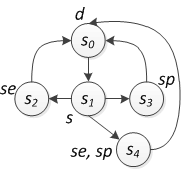
\includegraphics[width=4cm]{NnewCar.png}\\
		\caption{汽车制造企业模型}\label{BVM}
	\end{figure*}
\end{example}

日常生活中也有很多上述例子中的场景,如:商业交易过程、软件开发过程等~\cite{Baier:PMC:2008}。
但是对于给定原子命题的集合,从这些大型系统中“移除”掉这些原子而保持与这些原子无关的性质是一个复杂的问题。
此外,在这种情形下,两个重要的概念:最强必要条件(SNC)和最弱充分条件(WSC)问题也随之产生,其中SNC是指最一般的结论,WSC指最特殊的诱因。

基于上述存在的问题,本文在下面的研究意义部分给出对应的解决方案和其意义所在。

\subsection{研究意义}
在实际应用中,对于给定的$\Hm\models \varphi$问题,当$\Hm$满足$\varphi$时一般的验证器都会返回“yes”以表示满足,当$\Hm$不满足$\varphi$时验证器会给出一个使得$\varphi$不被$\Hm$满足的负例。此时,如何对$\Hm$进行修正使得其满足给定的规范是一个重要的问题。

最强后件(SP)和最弱前件(WP)(分别对应于上文提到的SNC和WSC)是形式化验证中的两个重要的概念,其不仅被用于汇编语言程序推理~\cite{legato2002weakest}和制定验证条件\cite{DBLP:journals/ipl/Leino05},还被应用于形式化验证过程中的负例生成\cite{dailler2018instrumenting}和系统精化(refinement)\cite{woodcock1990refinement}。
当$\Hm\not \models \varphi$时,若知道某个性质$\psi$使得若$\Hm$按照此性质进行修改后得到的新模型$\Hm'$能满足$\varphi$,即$\psi$为使得$\Hm\models \varphi$成立的充分条件($\Hm \models \psi\rto \varphi$)。
然而,现有的方法不能直接应用于计算当$\Hm$为不终止系统(如:反应式系统(reactive system))时使得“$\Hm\models \varphi$”为真的最强必要条件(SNC)和最弱充分条件(WSC)
(其详细原因将在下文指出)。此时,探索在$\Hm$下使得$\varphi$满足的定义在某个符号集合上的SNC和WSC将更进一步完善模型检测问题,
同时也为基于WSC的负例生成和精化提供了理论依据和新的计算方法。

此外,在上文中提到现有的方法不能直接应用于计算当$\Hm$为不终止系统时使得“$\Hm\models \varphi$”为真的最强必要条件(SNC)和最弱充分条件(WSC),在本文中将探索一种叫做\emph{遗忘理论}(forgetting)的方法来计算充分(必要)条件。正如下文将要说到的,遗忘理论作为知识表示与推理(KRR)中重要理论,具有较长的科研历史,且在许多逻辑中都有了较为成熟的研究。然而,在时序逻辑方面的研究目前还不成熟。因此,作为本文一个重要的研究意义,本文的研究将为时序逻辑下的遗忘理论的研究提供一个理论框架。
与此同时,借助遗忘理论计算上述形式化验证问题中的充分(必要)条件,这架起了KRR与形式化验证的桥梁。

\section{相关研究工作回顾}

遗忘(forgetting)是一种重要的知识抽取工具,它具有均匀插值(uniform interpolation)和二阶量化消解(second-order quantifier elimination,SOQE)两种称呼。
在很长一段时间内,遗忘被用于描述逻辑中本体(ontology)摘要的提取、敏感信息的隐藏和软件工程中计算两个文件的逻辑差(logic differences)。此外,其也被用于包括信念更新(belief update)、修改(repair)、规划(planning)和知识独立性的其他领域。

在规划中,遗忘主要用来计算其对应的后继状态公里所需要的SNC和WSC。下面就与本文密切相关的遗忘理论和SNC(WSC)进行详细的回顾。




差分隐私(differential privacy,DP)是一种严格的隐私保护模型,为个体隐私信息提供了强隐私保障。标准形式的差分隐私\cite{dwork2006differential,dwork2006calibrating}定义相邻兄弟数据集的查询输出结果满足概率$\epsilon$-不可区分性($\epsilon$-indistinguishability),其中$\epsilon$ 是足够小的非负实数。差分隐私利用随机化的方式能够实现在保护个体隐私信息的同时保持数据的统计信息
\cite{dwork2006differential,dwork2006calibrating,dwork2008differential},现已逐渐成为数据隐私的标准。通常,{\em 差分隐私被划分为中心化差分隐私和本地化差分隐私两种架构模式}\cite{dwork2014algorithmic}。中心化模型(centered model)假设系统中存在一个可信的数据管理者能够访问原始数据,并利用隐私保护机制得到扰动数据。与之对应的,本地化差分隐私(local differential privacy,LDP)\cite{kasiviswanathan2011what,duchi2013local}是差分隐私(DP)的本地化应用,它是系统中无可信数据管理者的特殊情景。其主要应用于隐私保护的数据收集场景。在本地模型(local model)中,每个用户本地的执行LDP 隐私协议扰动其真实数据得到扰动数据(perturbed data),并将扰动数据报告给数据收集者。然后,数据聚合者收集、存储、分析这些用户上报的扰动数据。当前,差分隐私已成为隐私保护研究的标准,对其应用的研究涉及社交网络\cite{wei2020asgldp,kasiviswanathan2013analyzing}、推荐服务\cite{xiao2020deep}、移动众包计算\cite{sei2017differential}等领域,%隐私保护的数据类型从关系数据延申至图数据、键-值型数据、地理数据等不同数据类别。
图\ref{fig:chapter02-application-research}描绘了差分隐私的主要应用领域和具体场景中的核心研究问题。
本文中,围绕个人数据生命周期阶段,结合差分隐私的具体应用场景,{\em 从隐私保护的数据发布、隐私保护的数据收集、隐私保护的数据分析}角度介绍目前国内外学术研究的动态与趋势。%随后,本文分析了在差分隐私的应用研究中需要关注的关键问题。

\begin{figure}[htbp]
	\centering
	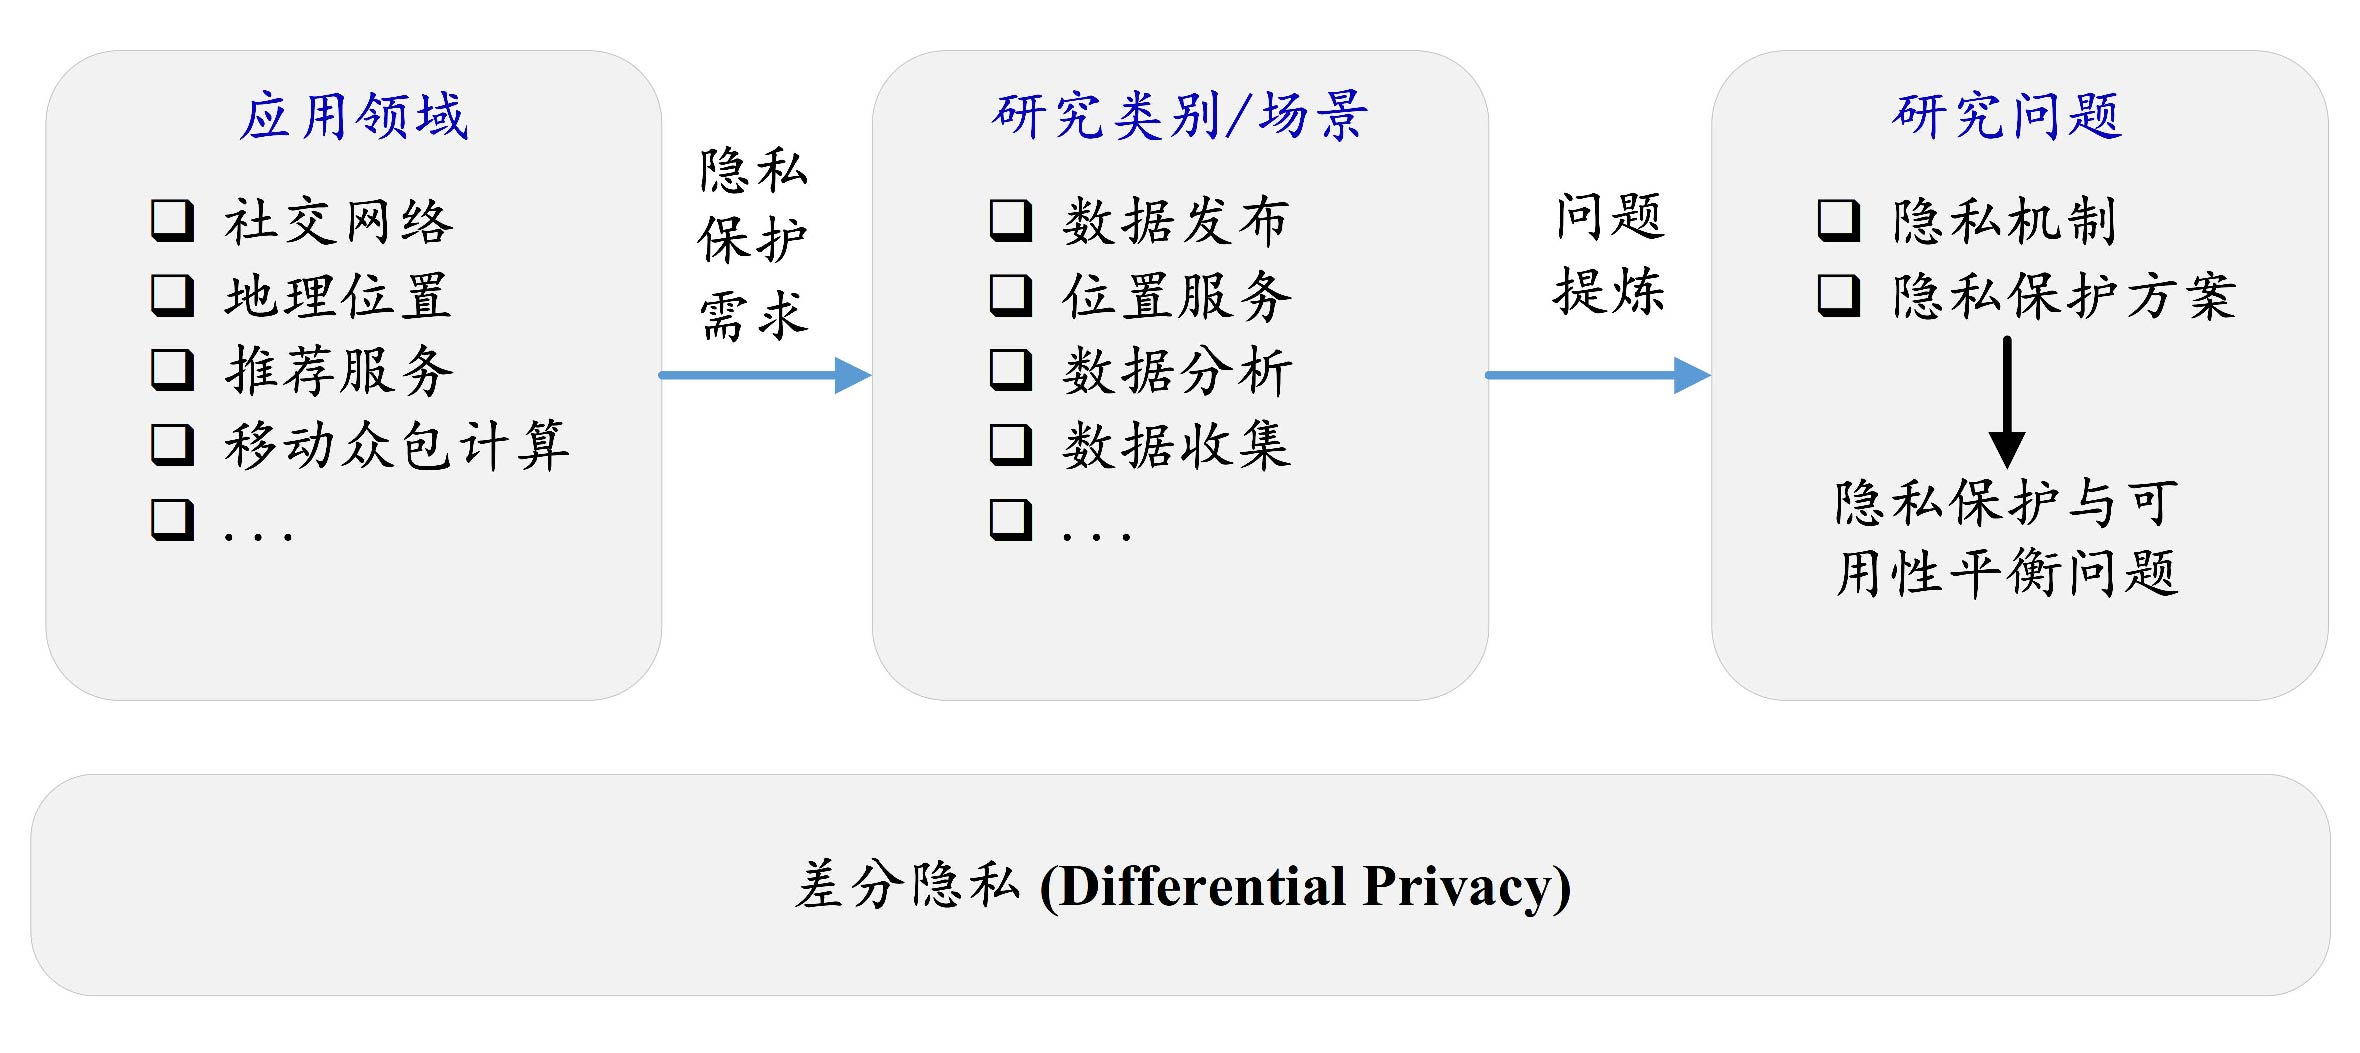
\includegraphics[width = 0.85\linewidth]{./figures/chapter02_3.jpg}
	\caption{差分隐私的应用研究}
	\label{fig:chapter02-application-research}
\end{figure}

接下来,综述近些年差分隐私应用研究中与本文研究相关的主要代表性成果,进一步分析差分隐私研究的发展趋势。

\subsection{遗忘理论}
遗忘这一词源于Lin等人关于一阶逻辑(first-order logic, FOL)工作~\cite{lin1994forget},在此之前的研究中多提到的是均匀插值~\cite{visser1996uniform,konev2009forgetting}和SOQE~\cite{ackermann1935untersuchungen}。

在命题逻辑中(propositional logic,PL),从公式$\varphi$里遗忘掉一个原子命题$p$通常记为$\Forget(\varphi,\{p\})$,得到的结果为$\varphi[p/\bot] \vee \varphi[p/\top]$(其与$\exists p\varphi$等价),其中$\varphi[X/Y]$为将$\varphi$中的$X$的全部出现替换为$Y$得到的结果。
%在Lin等人的文章中也将$\varphi[p/\bot] \vee \varphi[p/\top]$用$\exists p\varphi$来表示~\cite{lin1994forget}。
从公式中$\varphi$遗忘掉有限的原子命题的集合$P$被定义如下:
\begin{alignat*}{2}
	&  \Forget(\varphi, \emptyset) = \varphi, \qquad \\ % \nonumber
	&  \Forget(\varphi, P \cup \{q\})  = \Forget(\Forget(\varphi, \{q\}), P).
	\nonumber
\end{alignat*}

在FOL中,遗忘通常被看为SOQE问题的一个实例。
特别地,从FOL公式$\varphi$中遗忘掉一个$n$-元为此$P$得到结果为一个二阶公式$\exists R \varphi[P/R]$~\cite{lin1994forget}。
从这个角度看来,遗忘就是找到一个与二阶公式$\exists R \varphi[P/R]$等价的一阶公式。
然而,二阶逻辑的表达能力是严格大于一阶逻辑的,因而可以容易得出FOL下的遗忘不是封闭的,也就是说从有的一阶公式中遗忘掉某些谓词得到的结果不可以用一阶公式来表示。
作为FOL的一个子类,描述逻辑公式的遗忘也不总是存在的~\cite{DBLP:journals/ai/KonevL0W13},甚至对最基本的描述逻辑{\cal ALC}而言,遗忘的存在性问题都是不可判定的。
尽管如此,描述逻辑作为一种在语义网领域很重要的语言,其子类(包括{\cal ALCOHI}和{\cal ALCOIH})中的遗忘通常被用来抽取视图(review)~\cite{Wang:AMAI:2010,DBLP:conf/ijcai/LutzW11,Konev:JAIR:2012,DBLP:conf/ijcai/ZhaoS17,DBLP:conf/aaai/ZhaoSWZF20}。

现有的研究一阶逻辑和描述逻辑下的遗忘的方法有基于消解(resolution)和基于Ackermann引理的方法~\cite{DBLP:books/daglib/0023036}。
其中基于消解的方法是一种基于子句的归结反驳方法,消解规则是其基础。通常在这种方法中首先要把公式转换为其子句形式,然后再使用消解规则,最后将得到的子句集合中包含有要遗忘的谓词(原子命题)“移除”掉后得到结果可能就为遗忘的结果(在后文中会详细介绍与本文相关的消解规则和转换规则)。
基于Ackermman引理的方法主要是直接或间接(扩展)下面的Ackermann引理得到的。
\begin{lemma}[Lemma 6.1 of~\cite{DBLP:books/daglib/0023036}]
	给定关系变元$X$和一阶公式$\alpha(\overline{x}, \overline{z})$和$\beta(X)$,其中$\overline{x}$和$\overline{z}$为普通变元构成的多元组、$\overline{x}$中变元的个数与$X$的参数个数相同、且$\alpha$中不包括$X$。
	\begin{itemize}
		\item 若$\beta(X)$关于$X$是正的,即:$X$在$\beta(X)$中的每次出现前面都有偶数个“$\neg$”符号,则:
		$$\exists X \{\forall \overline{x} [X(\overline{x}) \rto \alpha(\overline{x},\overline{z})] \wedge \beta(X)\} \equiv \beta(X)_{\alpha(\overline{x},\overline{z})}^{X(\overline{x})}\hbox{。}$$
		\item 若$\beta(X)$关于$X$是负的,即:$X$在$\beta(X)$中的每次出现前面都有奇数个“$\neg$”符号,则:
		$$\exists X \{\forall \overline{x} [ \alpha(\overline{x},\overline{z}) \rto X(\overline{x})] \wedge \beta(X)\} \equiv \beta(X)_{\alpha(\overline{x},\overline{z})}^{X(\overline{x})}\hbox{。}$$
	\end{itemize}
\end{lemma}



\emph{知识遗忘}(knowledge forgetting)在模态逻辑S5中首先被提出并被用于推理智能体的知识状态(知识或者信念)~\cite{Yan:AIJ:2009}。
模态逻辑中的遗忘与经典逻辑下的遗忘不同,因为模态逻辑系统中引入了模态词,此时就不能以简单的谓词(命题)替换的方式获取遗忘的结果,如:
\begin{example}\cite{Zhang2008Properties}
	令S5公式$\varphi=\MPK p \wedge \neg \MPK q \wedge \neg \MPK \neg q$,则如果使用命题逻辑下的计算方法得到的结果为$\varphi[q/\top] \vee \varphi[q/\bot]$。
	这显然是不正确的,因为在遗忘$q$之后智能体的知识库不应该变得不一致。
\end{example}
为此,新的计算方法和四个能精确描述知识遗忘的基本条件被给出,值得注意的是这四个条件与知识遗忘形成了“当且仅当”的关系。换句话说,当知道某一个公式满足那四个条件则该公式为遗忘的结果,当知道某一结果为遗忘结果时它一定满足那四个基本条件。

均匀插值作为遗忘的一个对偶概念,这里有必要介绍一下模态逻辑系统的这一性质的研究现状。
S5、K和KD模态逻辑系统具有均匀插值性质~\cite{DBLP:journals/aml/Iemhoff19},
而模态逻辑系统没有均匀插值性质,如:模态逻辑量化的S5~\cite{DBLP:journals/jsyml/Fine79}和K4、和S4及其扩展都没有均匀插值性质~\cite{DBLP:journals/ndjfl/Schumm86},因此其遗忘也不是封闭的。
因此,在研究这些具有均匀插值性质的模态逻辑下的遗忘时可以借鉴S5系统下的遗忘方法,也可以参考K系统下的基于消解计算均匀插值的方法。
对于那些没有均匀插值的模态逻辑系统可以考虑模态逻辑下的Ackermann引理~\cite{DBLP:books/daglib/0023036}。


%此外,Feng等人也研究了S5下如

在非单调推理(non-monotonic reasoning)环境中,科研工作者们也从遗忘的基本条件的角度研究了
基于回答集语义的逻辑程序的遗忘,这些工作包括Zhang、Wang等人发表在AI和JAIR上的文章~\cite{DBLP:Zhang:AIJ2006,DBLP:journals/ai/EiterW08,Wong:PhD:Thesis,DBLP:journals/jair/WangZZZ14,wang2013forgetting,DBLP:journals/jair/Delgrande17,gonccalves2020limits},Eiter、Gonccalves等人的综述~\cite{eiter2019brief,gonccalves2021forgetting}。


%应用
在现实生活中,遗忘有很多应用。下面列出几点:
\begin{itemize}
	\item 计算后继状态公理:在规划问题中,根据最强必要条件和最弱充分条件有利于求出后继状态公理\cite{DBLP:journals/jair/Lin03}。在该文章中,最强必要条件和最弱充分条件都用遗忘来计算;
	\item 信息隐藏:在有的关键领域,为实现隐私保护,敏感信息必须被隐藏。而有的系统现在都基于本体,要做到隐私保护,只需要将那些敏感的概念(concept)和角色(role)符号隐藏(遗忘)就行了;
	\item 计算逻辑差:
	\item 知识更新:在许多场景,知识不是一层不变的,随着时间或空间的推移,会有新的知识加入,如何用新加入的信息更新原有知识而保证知识库的一致性是知识更新需要解决的问题。此外,知识更新也需要满足一些基本条件,在这些基本条件中,Katsuno和Mendelzon提出$(U1)-(U8)$较为常用,本文也使用这几个基本条件;
	\item 提取本体的概要:当一个本体工程师想要快速了解并测试一个本体的内容时,能事先快速地提取出该本体的概要是非常有用的。如果一个本体含有很多无关信息时,这将使得事半功倍。
\end{itemize}




差分隐私的基本思想是在隐私数据中引入随机性来阻止个人的信息被推断。显然地,随机化的程度越高,隐私保护效果越好,对应的数据可用性则降低。这就是隐私与效用原则\cite{sankar2013utility},也就是著名的隐私与效用权衡问题\cite{basciftci2016on,alvim2011differential}。该问题是隐私保护研究关注的核心问题,学术研究者围绕该问题做出了一系列有意义的研究工作。这些工作大致可以分为寻找更加有效的扰动机制\cite{ghosh2012universally,wang2016on,alvim2011differential}和研究有效的噪声注入方式\cite{geng2016the}两类。如文献\mycite{ghosh2012universally} 提出了几何机制(Truncated $\frac{1}{2}$-geometric mechanism)实现最优的差分隐私扰动。为了提高数据效用, 文献\mycite{xiao2011differential}提出在注入噪声之前,对数据进行小波变换(Wavelet Transforms),克服了Dwork方案中Laplace噪声扰动大的问题。文献\mycite{xu2017dppro}利用随机投影的方式研究了差分隐私高维数据发布的问题,解决了扰动误差大的问题。结合具体的应用场景,以下阐述差分隐私的学术研究动态。



首先,隐私保护的数据发布场景中,可信数据管理者发布数据以供进一步的数据分析\cite{aggarwal2008privacy},目标是发布数据的聚合信息而不泄露用户的个体隐私。差分隐私的数据发布包含有交互式发布和非交互式发布两种类型,其中,交互式数据发布包含有事务型数据发布、直方图数据发布、流数据发布、图数据发布;非交互式数据发布主要有批量查询发布、合成数据集发布\cite{zhu2017differentially}。隐私保护的数据发布场景中,发布数据的精确度与隐私泄露权衡是主要关注的核心问题。{\em 为了解决数据发布中存在的隐私泄露问题,差分隐私的机制是研究的核心关注点}。近年来,以Dwork的方法
\cite{dwork2006calibrating}为基础,针对不同的发布数据类型,研究者提出了诸多的差分隐私数据发布模型及算法。
表\ref{tab:survey_dp_publishing}列出了差分隐私数据发布的主要部分研究工作。

\begin{table}[htbp]
\caption{差分隐私的数据发布方法}
\label{tab:survey_dp_publishing}
\centering
\fontsize{10pt}{\baselineskip}\selectfont
\begin{tabular}{p{0.10\textwidth}p{0.05\textwidth}p{0.30\textwidth}p{0.30\textwidth}}
\toprule
	\textbf{工作模式}& &\textbf{数据发布类型}&\textbf{主要研究}\\
	\midrule
   交互式数据发布& &\makecell[l]{事务型数据发布 \\ 直方图数据发布 \\ 流数据发布\\ 图数据发布} &\makecell[l]{
IDC\cite{gupta2012iterative}\\Laplace\cite{dwork2006calibrating},Partitioning\cite{chen2011publishing}\\ Pan-Privacy\cite{dwork2010differential},P-Sums\cite{chan2011private}\\ Edge DP\cite{zhang2015private}, Node DP\cite{kasiviswanathan2013analyzing}} \\
   \midrule
非交互式数据发布& &\makecell[l]{批量查询发布\\ 合成数据集发布} & \makecell[l]{Batch Query\cite{yuan2012low}\\ Sanitization\cite{dwork2009on}}\\

  \bottomrule
\end{tabular}
\end{table}

其次,本地化差分隐私的应用研究\cite{yeqingqing2018}已逐渐成为差分隐私的另一个重要研究方向,在隐私保护的数据收集、数据发布场景中都得到了不同程度的应用。围绕本地化差分隐私的应用,主要是研究如何设计可获得的隐私机制实现预期的目标。本地隐私模型中,随机化响应(Randomized Response,RR)\cite{warner1965randomized}技术是一种获得LDP的有效方式,现已发展成为本地化差分隐私机制设计的基本构建模块,在本地差分隐私中的应用取得了显著的效果。近年来,很多著名的LDP隐私机制(如$k$-RR \cite{kairouz2016extremal},$O$-RR\cite{kairouz2016discrete},RAPPOR \cite{erlingsson2014rappor,fanti2016building},MeanEst\cite{duchi2013localprivacy}等)已经被研究者提出。周异辉等\cite{zhouyihui2019}针对隐私-效用均衡问题,从优化理论的角度给出了效用优化模型,并分析了随机响应机制的最优性条件和相应的效用最优机制。此外,对于其它数据结构的本地化差分隐私也得到了研究,如set-value的本地化差分隐私
\cite{wang2018privset,qin2016heavy}、key-value类型数据的本地化差分隐私\cite{ye2019privkv}以及图数据结构的本地化差分隐私\cite{wei2020asgldp}。本地化差分隐私的应用涉及到社交网络\cite{qin2017generating}、移动众包计算\cite{sei2017differential}、数据合成发布\cite{ren2018textsf,yang2017copula}等场景,也因此日渐受到关注。本地化模型中,攻击模型通常被假设为半诚实(Semi-honest)的敌手模型,也就是说,数据聚合者诚实的执行隐私协议但是试图从报告的扰动数据中推断用户个体的隐私信息\cite{sei2017differential}。在本地化模型中,隐私与效用的权衡问题仍然是学术研究关注的重点。

最后,隐私保护的数据分析是在保持数据分析的精确度的同时保护个体的隐私信息\cite{wang2016on}。近年来,基于学习理论的方法在差分隐私中得到了具体的应用,包括数据分析与机器学习的方法在差分隐私中的应用\cite{kasiviswanathan2011what,ye2017optimal,sarwate2013signal}(如概率分布估计\cite{Murakami2018Toward},数据训练\cite{xu2019ganobfuscator})。2018年,Ren 等\cite{ren2018textsf} 使用~(Expectation Maximization,EM)~和~Lasso~的方法进行分布估计,用于得到联合概率分布,支撑发布数据集合成。2019年,Wang等\cite{wang2019collecting}基于机器学习的线性回归(Linear Regression)、逻辑回归(Logistic Regression)、支持向量机(Support Vector Machines,SVM)分类算法分析了所提出分段机制(Piecewise Mechanism,PM)和混合机制(Hybrid Mechanism,HM)的性能。由此可知,隐私保护的数据分析主要是学习数据的统计特征,体现出扰动数据的质量。

鉴于上述分析可知,差分隐私在隐私保护中占据着重要的地位,它已经涉及到了具有隐私保护需求的各种信息系统应用。现阶段,差分隐私在面向低维数据和独立同分布数据情景的研究相对比较成熟。针对低维的数值型数据和类别型数据,目前已有诸多的隐私保护方案(如Duchi等人\cite{duchi2018minimax}提出的数值型方案,Wang等人\cite{wang2017locally}提出的类别型Optimized Unary Encoding,OUE方案)。但是,随着应用系统的需求升级,面向多维数据且存在数据关联的情景时,直接地拓展当前的方案到多维情景,则会面临性能和效用降低的挑战。此外,多维属性的用户隐私敏感偏好表达也是亟待解决的问题。针对这些问题,研究者积极的探索新的解决方案,以下给出研究进展及现状的介绍。



(1) {\em 面向多维数据的差分隐私}

随着用户数据维度的增加,多维或高维数据具有笛卡尔乘积空间大、数据稀疏性的特点,给差分隐私数据处理带来新的挑战。具体地说,差分隐私对于多维数据或高维数据的处理主要面临着隐私脆弱性、计算复杂度高等问题。为了解决这些问题,数据降维是一种通常采用的处理方法。将有关个体的数据元组,拆分为多个属性分量,然后独立的应用差分隐私机制,该处理思想以差分隐私的并行组合原理\cite{dwork2014algorithmic}为基础,其基本的处理流程如图\ref{fig:chapter02-multidimension-data}描述。

\begin{figure}[htbp]
	\centering
	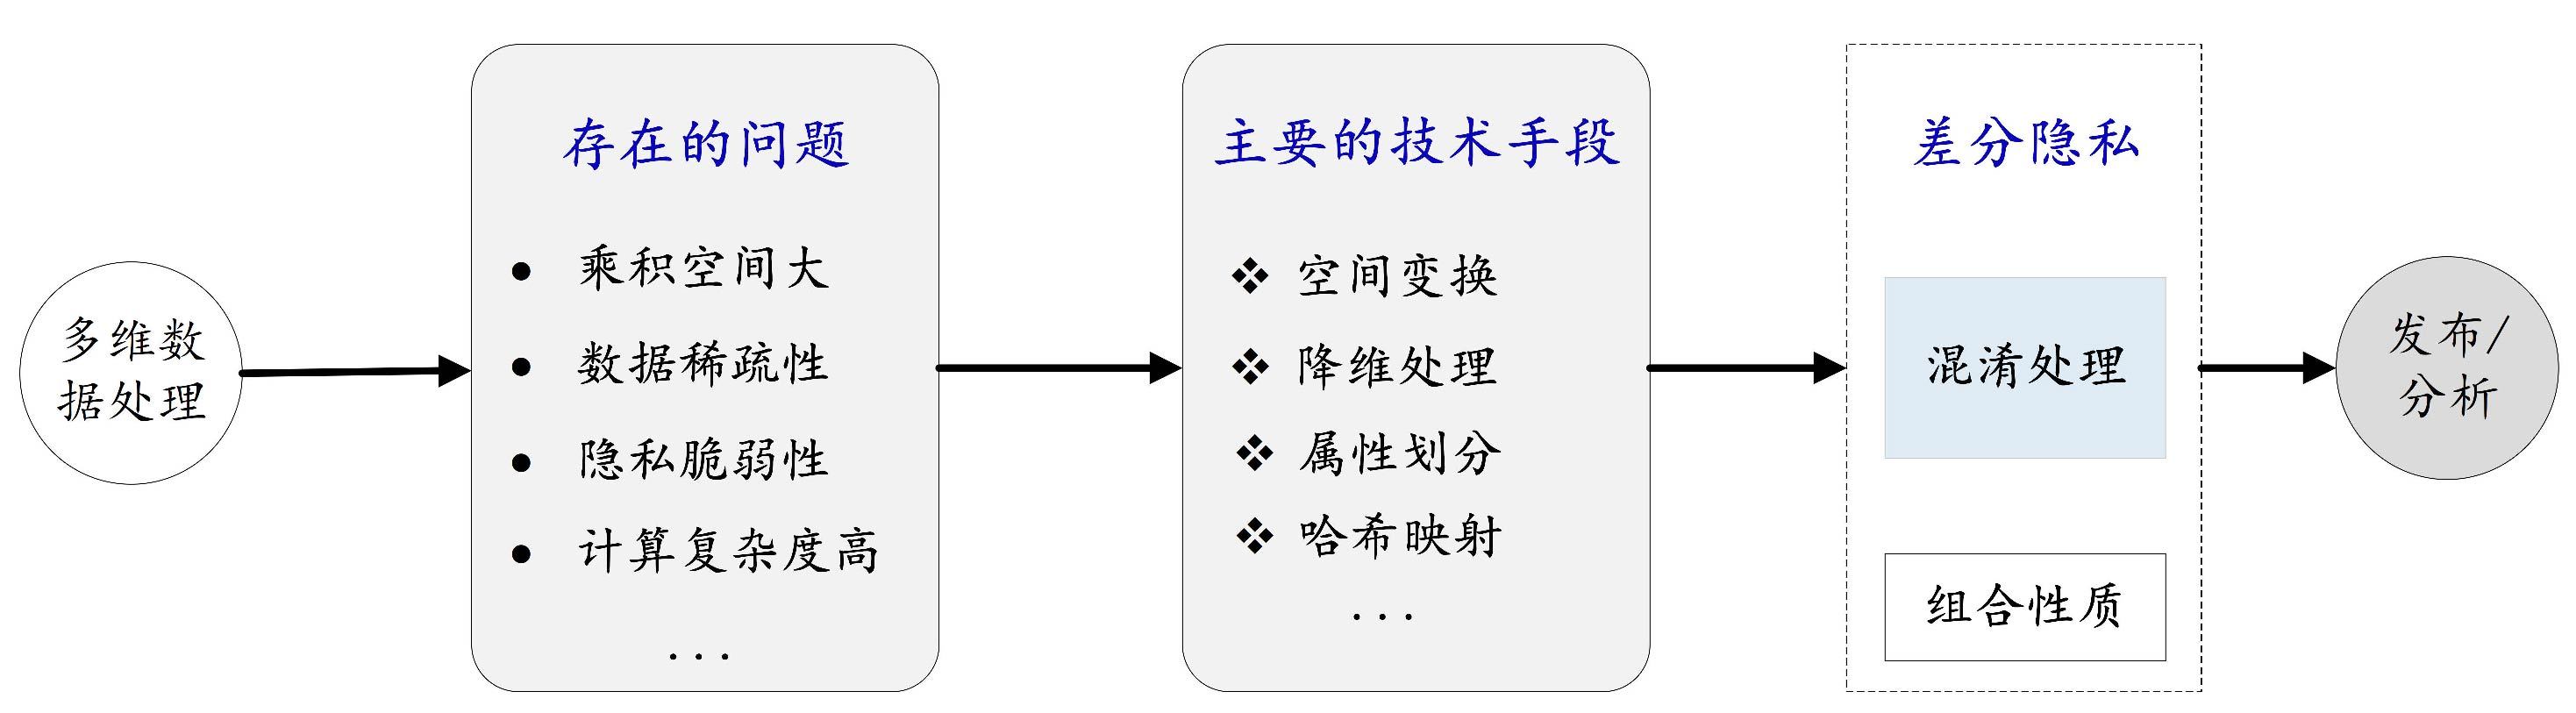
\includegraphics[width = 0.85\linewidth]{./figures/chapter02_4.jpg}
	\caption{差分隐私多维数据处理流程}
	\label{fig:chapter02-multidimension-data}
\end{figure}

针对差分隐私的多维数据处理,研究者做了一些有意义的探索,提出了差分隐私的多维数据处理方案。2017年,Xu等\cite{xu2017dppro}针对多维数据发布中存在的扰动误差增加和计算复杂性问题,通过随机投影的方法提出了高维数据发布的DPPro方案。此外的本地化差分隐私模型中,Wang等\cite{wang2019collecting}针对多维数据的收集和分析场景,推广并改进了Duchi等人\cite{duchi2018minimax}的方案,提出了分段机制(PM)和混合机制(HM),其思想是将属性分为数值型和类别型数据,然后依赖于单一数值型扰动方案和存在的任意类别型扰动方案(如OUE\cite{wang2017locally}),实现多维混合数值型和类别型数据的处理。Ren等\cite{ren2018textsf}将基于Bloom Filter和RR实现的RAPPOR机制拓展应用到高维数据情景,利用属性值拆分、扰动合并和差分隐私的组合定理\cite{kairouz2017the},考虑了差分隐私高维数据发布的问题,提出了LoPub。其基本思想是将元组进行属性拆分,然后利用Hash函数和Bloom Filter映射属性值到比特串,并逐比特的进行随机扰动,产生扰动的元组。该方法首先将原始数据哈希得到``0''和``1''的比特串,然后随机响应实现随机的扰动。Yang等\cite{yang2017copula}基于随机响应技术本地转化用户数据到比特串,实现多维数据合成和发布的机制。事实证明这是一种相对有效的处理方法,且被广泛的应用在隐私保护的多维数据情景。该思想在基于地理位置的隐私保护系统中也有相应的应用。如混淆扰动一个元组时,独立的应用存在的隐私保护机制到元组的每一个位置点,然后得到整个响应的混淆元组\cite{andres2013geo}。近年来,面向多维数据的差分隐私研究逐渐成为一个重要的研究点,但是,目前针对混合数值型和类别型多维数据处理的差分隐私最优化机制的研究还相对较少。面向多维数据处理的差分隐私机制设计仍然是一个重要的研究方向,尚需要进一步的研究。


(2) {\em 面向数据关联的差分隐私}

现有的差分隐私处理方法大多假设数据抽样独立,然而实际应用中,多维数据通常不是独立存在,而是存在着相互关联的情况。事实上,这些关联可以分为数据的记录关联、属性关联或隐私攻击者的关联辅助背景知识关联等情况。文献\mycite{kifer2011no}揭示了相关数据上的隐私机制将比期望的泄露更多的信息。为此,近些年数据关联的差分隐私机制设计问题受到研究者关注。

{\em 例如,数据集中属性年龄、职业可能和婚姻状态存在属性关联,这种关联使得敌手能够以较高的置信推断用户的隐私信息,从而增加隐私泄露风险。针对数据关联隐私泄露问题,文献}\mycite{zhu2015correlated}{\em 揭示由属性导致的元组相关,增加了流感疾病隐私泄露风险;文献}\mycite{li2019impact}{\em 分析了敌手背景知识对隐私泄露的影响。}针对数据关联的隐私泄露影响,研究者开展了相关的研究工作。
2014年,Zhang 等\cite{zhang2014privbayes}利用贝叶斯网络考虑了数据集属性关联的情景,借助互信息分析属性之间的相关度\cite{reshef2011detecting,liangjy2016},提出利用贝叶斯网络实现差分隐私的高维数据发布。2015年,Zhu等\cite{zhu2015correlated}针对非独立同分布的数据集记录关联,改进了差分隐私的敏感度计算方法,减少了噪声注入提升了数据效用。Yang等\cite{yang2015bayesian}研究了数据相关对隐私的影响,敌手先验知识对隐私的影响和数据相关时的扰动算法设计,提出了贝叶斯差分隐私。2017年,Song等\cite{song2017pufferfish}提出Pufferfish privacy保护关联数据的隐私。2019 年,Li 等\cite{li2019impact} 基于皮尔逊的相关度分析方法,从强关联、弱关联、正相关和负相关的角度,考虑了隐私攻击者的背景知识和数据关联对差分隐私数据发布的影响。鉴于上述分析,由数据的记录关联、属性关联或隐私攻击者的关联辅助背景知识,导致的隐私泄露问题,或是存在数据关联的高维数据发布问题仍然是学术研究关注的焦点。数据相关的隐私度量分析成为隐私机制设计首要解决的问题。

(3) {\em 面向用户偏好的差分隐私}

差分隐私模型扩展应用于多维数据时,差分隐私的隐私特性($\epsilon$-度量)由其组合性质保障。通常情况下,差分隐私把多维属性看作等价敏感,提供相同等级的隐私保护。例如,用户个体的隐私数据包含$d$个属性维度,差分隐私机制的隐私预算设置$\epsilon/k$,然后依据序列组合性质,隐私保护总体满足$\epsilon$- 差分隐私。但是,多维的属性之间可能存在不同的隐私敏感度,也就是用户的隐私敏感偏好。为了更好的阐述这个问题,首先给出以下问题引例。

{\em 假设个体数据元组由年龄、性别、教育程度、婚姻状态组成,这些数据项都是有关个体的隐私信息。但是,在这些数据项中,用户对其数据具有不同的隐私感受。通常情况下,一个人的性别可能不被认为是隐私数据或者具有较低的隐私敏感性。然而,一个人的婚姻状态(如离婚)是想保持私密性的敏感数据,其隐私私密性高于其它属性。}为了能够解决诸如此类的问题,这就要求差分隐私能够提供不同敏感等级的隐私保护对于有区分的属性,满足所提出的隐私保护需求。

针对上述问题,研究者依据属性敏感度等级,提出了有区别隐私数据的个性化差分隐私保护方案\cite{chen2016private}。2015年,Jorgensen等\cite{jorgensen2015conservative}考虑个人数据的不同隐私保护需求,提出了个性化差分隐私(Personalized Differential Privacy,PDP)的概念。2019 年,Wang 等\cite{wang2019personalized}利用泛化的$d_{\mathcal{X}}$-privacy\cite{chatzikokolakis2013broadening}研究了个性化隐私保护。Murakami 等\cite{murakami2019utility} 提出了效用最优的本地化差分隐私方案(Utility-optimized LDP,ULDP)用于隐私保护的数据收集与分析。通过划分个体数据为敏感数据和非敏感数据两部分,推广Mangat\cite{mangat1994an}随机响应到多元字母表情景,提出了ULDP方案,对于敏感数据提供和LDP 等价的隐私保障。2020年,Gu 等\cite{gu2020providing}通过考虑不同输入数据具有不同的隐私敏感度,提出了一种输入区分(Input-discriminiative)的隐私保护机制(Input-discriminiative LDP,ID-LDP)。由此可见,考虑用户隐私偏好,设计差分隐私机制,实现为不同敏感度的用户数据提供有区分的隐私保护成为一种新的研究方向。


\subsection{SNC和WSC}
Shannon\cite{shannon1948a}为解决信息度量问题提出信息熵的概念之后,信息熵在通信、密码学等领域发挥了重要的作用。近年来,基于信息度量的量化信息流思想(Quantitative Information Flow,QIF)\cite{smith2009on}逐渐在隐私保护中得到应用。此外,博弈均衡理论作为一种有效的分析工具在隐私保护中也得到了应用。针对差分隐私应用中存在的隐私与效用的平衡问题,基于信息论、博弈论以及交叉学科的方法开展研究逐渐成为一个重要的研究方向。以下从两个方面综述密切相关且具有代表性的研究成果。

(1) {\em 差分隐私的信息论方法}\label{subsec:information_dp}

隐私保护模型的本质是数据混淆、扰动机制,它可以表达为一种概率性的函数映射,与信息论的方法密切相关\cite{Duchi2019information}。由此,在隐私保护研究中,信息熵发展成为一种有效的隐私度量方法\cite{issa2016an,Chatzikokolakis2008Anonymity}。以信息熵为基础定义的R\'{e}nyi熵\cite{renyi1961on,erven2014renyi,mironov2017renyi}、条件熵、联合熵、互信息量等在隐私保护研究中得到了应用\cite{wang2019consistent,mcgregor2010the,du2015Fundamental,lopuhaa-zwakenberg2019information}。{\em 首先,隐私度量方面},Mir 等\cite{mir2012information}利用信息熵、条件熵、互信息量研究了隐私信息的度量问题,奠定了差分隐私的信息论方法研究基础。Barthe 等\cite{barthe2011information} 利用信息熵研究了差分隐私的隐私边界问题。Issa等\cite{issa2016an,2016Maximal}提出Maximal leakage方法测量隐私泄露,随后,Liao等\cite{liao2019tunable}对其扩展提出$\alpha$-leakage。{\em 其次,信息论的方法对于差分隐私的机制研究}也有一定的应用\cite{diaz2020on,kairouz2016extremal,wang2016on}。2011年,Alvim 等\cite{alvim2011differential,alvim2011on,alvim2015on}几乎是最早提出基于量化信息流(QIF) 的思想,将信息熵应用到差分隐私中量化隐私信息的不确定度,抽象差分隐私噪声机制为信息论噪声信道,并从信息论的角度考虑了平衡隐私度与数据效用的方法,同时提出信息论对称信道机制能够达到理论上的最优性。{\em 随后,信息论方法研究的差分隐私与标准差分隐私之间的关系}得到研究者关注\cite{mcgregor2010the}。Cuff 等\cite{cuff2016differential}基于互信息的概念给出了与标准差分隐私等价的信息论差分隐私定义。文献\mycite{calmon2012privacy,makhdoumi2013privacy}研究建立了互信息约束与差分隐私的关系。进一步,Wang 等\cite{wang2016on}提出可辨识识别(Identifiability)的概念、并研究了与差分隐私(Differential Privacy) 和互信息隐私(Mutual Information Privacy) 三个不同隐私概念之间的基本联系。{\em 更重要地是,信息论中著名的信源编码定理、限失真编码定理(保真度准则)}\cite{cover2006elements}{\em 在隐私保护中均得到了相应地研究}\cite{rebollo-monedero2010from,du2015Fundamental}。如Sankar等\cite{sankar2013utility}针对统计数据库隐私泄露问题,构建了统计数据库的概率模型,从最佳信源编码、译码方案的角度考虑了信息论方法在数据库中平衡隐私与效用的应用。在允许部分失真的情况下,最小信息传输率的率失真理论在差分隐私\cite{mir2012information,wang2016on}最优机制研究中也受到了关注。

随机响应技术是实现本地化差分隐私的有效方法,信息论方法对于随机响应的研究也得到了广泛的应用。事实上,本地化差分隐私的随机响应实现是根据特定的概率密度函数(Probability Density Function,PDF)随机响应。在此方面的研究关键在于设计满足差分隐私的概率密度函数。{\em 近年来,信息论方法的研究已从二元随机响应发展到多元随机响应,逐步向复杂数据类型拓展延伸}。具体的研究工作从信息论的本地化差分隐私度量
\cite{lopuhaa-zwakenberg2019information},向最优机制设计发展。Sarwate 等\cite{sarwate2014a}抽象二元离散随机响应机制为Shannon 信息论\cite{shannon1948a}离散噪声信道,基于率失真理论\cite{cover2006elements} 对本地化差分隐私的二元随机响应机制进行了研究,指出对称信道机制能达到最优性。但是,二元随机响应仅能处理`` 是''和``否''的问题,其应用具有局限性。随后,研究者对其进行了拓展研究,发展了多元随机响应(Multivariate Randomized Response,MRR) 技术。Kairouz等\cite{kairouz2016extremal} 基于互信息提出了$k$-RR机制,并在此后被进一步研究,发展了一系列先进的差分隐私机制。Kalantari 等\cite{kalantari2018robust}考虑不同先验概率分布情况,研究了汉明失真下平衡隐私度与数据效用的最佳差分隐私信道机制问题,指出对称信道机制和非对称信道机制的最优性对不同分布的最优性。Xiong 等\cite{xiong2016randomized}在隐私保护的数据收集场景,利用信息论的方法,将差分隐私的数据扰动机制抽象为离散无记忆的噪声信道机制,从限失真约束条件定义差分隐私信道集合,研究了本地化差分隐私的机制问题。

{\em 基于这些相关的研究工作,可以看出信息论的方法应用于差分隐私研究,主要是解决两个方面的问题}:(1) {\em 隐私信息的度量问题};(2) {\em 差分隐私的机制设计问题}。首先,前者的研究主要是从熵的内涵角度理解隐私泄露问题,该研究可用于评估隐私泄露风险(例如,定量分析隐私泄露的界),同时也是信息论方法对差分隐私机制研究的基础;其次,为了解决隐私与效用的平衡问题,后者的研究主要关注于最优的差分隐私实现机制。对于该问题的解决,信息论方法是从噪声信道角度寻找满足给定约束条件的最优条件概率分布。由此,基于优化理论建模\cite{iyengar2019towards}、求解该问题是一种理想的选择。如极大极小定理、Karush-Kuhn-Tucker (KKT)条件等\cite{boyd2004convex}得到了具体的应用。结合凸性或拟凸性形式化隐私与效用平衡问题为拟凸优化问题\cite{xiong2016randomized}、隐私失真最优化问题\cite{wang2016on}(信息论领域的率失真问题)
是较好的解决方法。但是,现阶段信息论方法总是假设数据抽样独立,对多维数据情景、多维属性存在关联、混合数值型和类别型的最优差分隐私机制问题尚未充分研究。

(2) {\em 差分隐私的博弈论方法}

隐私与效用的平衡问题(Privacy-utility Tradeoff)是隐私保护数据收集、隐私保护数据发布等应用场景中广泛关注的矛盾冲突问题。直观地,隐私保护效果越好,则噪声扰动导致的数据质量损失越大,从而数据效用降低。反之,数据效用越高,则隐私保护强度减弱,由此引发的隐私泄露量较大,这被称为隐私与效用原则\cite{sankar2013utility}。在隐私保护的模型与算法研究中,如何平衡隐私与效用是一个研究的关键问题。针对此,上述优化理论的方法是一种行之有效的解决方案。除此之外,基于最优性发展起来的博弈论\cite{Neumann1944The}也为隐私保护提供了有效的分析手段。博弈分析方法从理性的角度分析存在矛盾冲突情景下的参与者最优策略选择问题。近年来,在差分隐私研究中得到了一定程度的应用,其基本思想是分析隐私保护系统中参与者的理性行为,以均衡的思想解决隐私保护与数据效用平衡问题。

2013年,Hsu等\cite{hsu2013differential} 在差分隐私框架下针对隐私查询发布问题,建立了数据拥有者和数据查询者之间的两方零和博弈模型,提出一种新的隐私机制。2017年,Wu等\cite{Wu2017Game}构建了一个多方的有限策略型博弈,利用纯策略纳什均衡的存在性条件\cite{Glicksberg1952A}研究了差分隐私关联数据集发布的隐私预算参数选取问题。2019年,Qu等\cite{cui2019improving}针对隐私与数据效用之间的权衡问题,提出了一种基于社会距离的个性化差分隐私方法,在用户和敌手之间建立了静态贝叶斯博弈,从贝叶斯纳什均衡的角度权衡隐私与效用。此外,非合作的微分博弈\cite{gao2019a}和斯坦伯格博弈(Stackelberg)\cite{fioretto2020differential,shokri2015privacy} 也都在差分隐私中得到了研究。值得强调的是,Alvim 等\cite{alvim2017information,alvim2018leakage}基于量化信息流的思想,采用信息论方法度量隐私泄露,构建了隐私保护攻击与防御的两方零和博弈模型,进一步,基于极大极小理论\cite{du1995minimax}分析了隐私防护者与隐私攻击者的最佳策略选择。该研究工作将信息论的方法融入到博弈模型中,标志着一种新的研究趋势。但是,该研究工作没有针对具体的差分隐私保护模型展开研究,因此,在该方面仍然存在较大的研究提升空间。博弈模型用于差分隐私的研究,关键问题在于分析具体应用场景中隐私保护参与者和策略集,定义合理的收益函数,解决均衡的问题。

\section{研究目标及主要结果}

相关研究工作表明现存方法不能很好的解决反应式系统下的WSC(SNC)的求解。然而,WSC是一种进行系统修改的重要知识,寻求一种有效的求解方法有利于系统正确性的确保。
在知识表示与推理中,一种叫做遗忘的技术可以用于求解给定理论(公式)的WSC(SNC)。
但是,就如上面所述时序逻辑下的遗忘理论尚处于不成熟阶段,没有一个统一的理论框架。
此外,如何用遗忘来计算给定系统模型和性质的WSC(SNC)也是一个重要问题。

基于此,{\em 本文从遗忘理论的角度出发,拟研究反应式系统的SNC和WSC的计算,从而为计算不终止类系统下的定义在某个符号集上的SNC和WSC提供了新的方法,架起形式化验证与KRR之间的桥梁。}
%特别地,本文将规范的描述语言限制到$\CTL$和$\mu$-演算下。
为了实现这一目标,本文\textbf{主要研究内容及结果}如下:

(1) {\em $CTL$和$\mu$-演算的遗忘理论}

本文研究了$\CTL$中遗忘理论的方法和性质,特别是其遗忘结果的存在性、复杂性等,为探索用遗忘理论计算SNC和WSC提供理论基础。具体说来,遗忘理论具有削弱(Weakening,(W))、正维持(Positive Persistence,(PP))、负维持(Negative Persistence,(NP))、无关性(Irrelevance,(IR))等基本性质\cite{Yan:AIJ:2009}。本文探索$\CTL$和$\mu$-演算的遗忘理论的以上性质,并探讨其与存在性之间的关系。此外,本文深入研究了 $\CTL$和$\mu$-演算 遗忘理论的基本准则、发现计算$\CTL$和$\mu$-演算遗忘结果的算法以及探讨$\CTL$和$\mu$-演算子类与遗忘相关问题的计算复杂度,为研究计算SNC和WSC的性质、算法以及基本准则等作好铺垫。具体说来,有以下两点:
\begin{itemize}
	\item \textbf{$\CTL$的遗忘理论:}
	$\CTL$不具有均匀插值(uniform interpolation)性质\cite{Maksimova:JANCL:1991},即:不存在一个算法使得对于任意的$\CTL$公式,其遗忘掉任意原子命题的集合得到的结果仍然是$\CTL$公式。在这种情况下,本文除了探讨了上述$\CTL$中遗忘的性质,还研究了$\CTL$子类的遗忘理论,特别是能保证其遗忘结果仍然是$\CTL$可表达的子类。在这些子类中,一个特殊的子类为约束$\CTL$(bunded \CTL)。在这种情形下,每个公式的模型是有限个数个,且每一个模型都能用一个$\CTL$表示。因此,其遗忘理论是封闭的。
	
	\item \textbf{$\mu$-演算的遗忘理论:}
	与$\CTL$不同,$\mu$-演算虽然表达能力比$\CTL$强,其可满足性问题也比$\CTL$的复杂,但是$\mu$-演算具有均匀插值性质\cite{DBLP:DAgostino:JAL:2006}。这意味着对于在任意的$\mu$-演算句子中遗忘掉任意的原子命题的集合得到的结果仍然是$\mu$-演算公式。本文给出了$\mu$-演算下遗忘理论的主要框架:包括上述遗忘理论的性质和计算遗忘的方法。
	特别地,表明了本文提出的$\mu$-演算下的遗忘定义与均匀插值是一对对偶概念,即本文中的遗忘理论的性质也是均匀插值的性质,这位研究均匀插值提供了另一种途径。
	此外,本文还说明了当$\mu$-公式为吸取$\mu$-公式时,计算遗忘理论可以在多项式时间内完成,这为$\mu$-演算下的遗忘的计算提供了一种有效的方法。
\end{itemize}


(2) {\em $CTL$下遗忘理论的算法的研究及实现}

基于上述研究结果,设计并实现一个计算$\CTL$和$\mu$-演算遗忘结果的原型系统,并从实验角度研究其计算代价以启发快速的计算遗忘结果的算法。
具体说来,本文给出了一种基于消解的计算$\CTL$遗忘的算法,并使用Prolog实现了该算法。

(3) {\em 遗忘理论在形式化验证和知识更新中的应用}

给出了使用遗忘理论计算给定有限系统模型的SNC和WSC。如上所述,一个有限的系统模型能够被一个$\CTL$公式描述,因而可以使用遗忘理论计算其SNC和WSC。
此外,知识更新是一种使用新发现的性质更新已有理论的技术,本文探讨了如何使用遗忘理论更新$\CTL$和$\mu$-演算下的理论。
表明了使用遗忘理论定义的知识更新满足现有的知识更新的八条准则。

~\\
针对上述几个内容,解决了以下4个\textbf{关键问题}:

(1) {\em $\CTL$的遗忘什么情形下存在?如何计算遗忘?}

$\CTL$是一种分支时序逻辑,已有文献表明$\CTL$不具有均匀插值性质。与此同时,$\CTL$还引入了时态算子(temporal operator)。在此情形下,研究$\CTL$的遗忘就不能像已有的经典命题逻辑和模态逻辑S5那样,因为遗忘与均匀插值是一对对偶概念,即:它们可以互相证明彼此的存在性。为此,本文深度刨析现存的消解规则,提出了一种基于消解的计算遗忘的方法。该方法表明,当所有在转换为$\CTL$标准形式过程中引入的新的原子命题都被“消除”掉时,使用这一方法得到的结果即为遗忘的结果,即:这一方法是可靠的。
尽管$\CTL$的遗忘理论不是封闭的,但是本文给出:当被消解的原子命题只能同时出现在同一模态词下的命题公式里时,遗忘总是存在的。

此外,考虑到现实生活中有的情形下只需要考虑有限模型,所以本文研究了约束$\CTL$下的遗忘理论。研究表明,这种情况下的遗忘结果可以由有限个模型的特征公式(一种$\CTL$公式)的吸取来表示,从而说明了这种情形下的遗忘是封闭(存在)的。

(2) {\em 遗忘理论与反应式系统的SNC和WSC的关系}

在经典命题逻辑和一阶逻辑中,遗忘理论与SNC和WSC的关系分别已经被Lin 和 Doherty等人分别提出[22][23]。特别地,经典命题逻辑中的SNC和WSC被用于规划问题中的后继状态公理的计算。这里所说的SNC和WSC都是在给定的命题公式或一阶公式下的。本文给出,当给定一个有限反应式系统(Kripke structure)时,将该系统表示为其特征公式时就可使用
上述所说的$\CTL$和$\mu$-演算的遗忘理论计算SNC和WSC。



(3) {\em $CTL$和$\mu$-演算的遗忘在推理问题上的复杂性}

计算复杂性理论致力于将可计算问题根据它们本身的复杂性分类。研究表明,在经典命题逻辑中:CNF(Conjunctive normal form)公式的遗忘的推理问题最难是$\Pi_2^P$完全的,DNF(Disjunctive normal form)公式的遗忘的推理问题是co-NP-C的;在模态逻辑S5中,遗忘的模型检测问题是NP-C的,对应的推理问题是$\Pi_2^P$完全的。基于此,本文从现有复杂性结果和自动机理论研究$\CTL$和$\mu$-演算的遗忘在模型检测和推理问题上的复杂性。








\section{论文组织结构}
本文研究了差分隐私数据发布、数据收集场景中隐私与数据效用权衡的差分隐私均衡优化模型与算法。全文共分为七章,组织结构如图\ref{fig:chapter1-research-structure}所示,各章节内容的具体安排如下:

\begin{figure}[htbp]
	\centering
	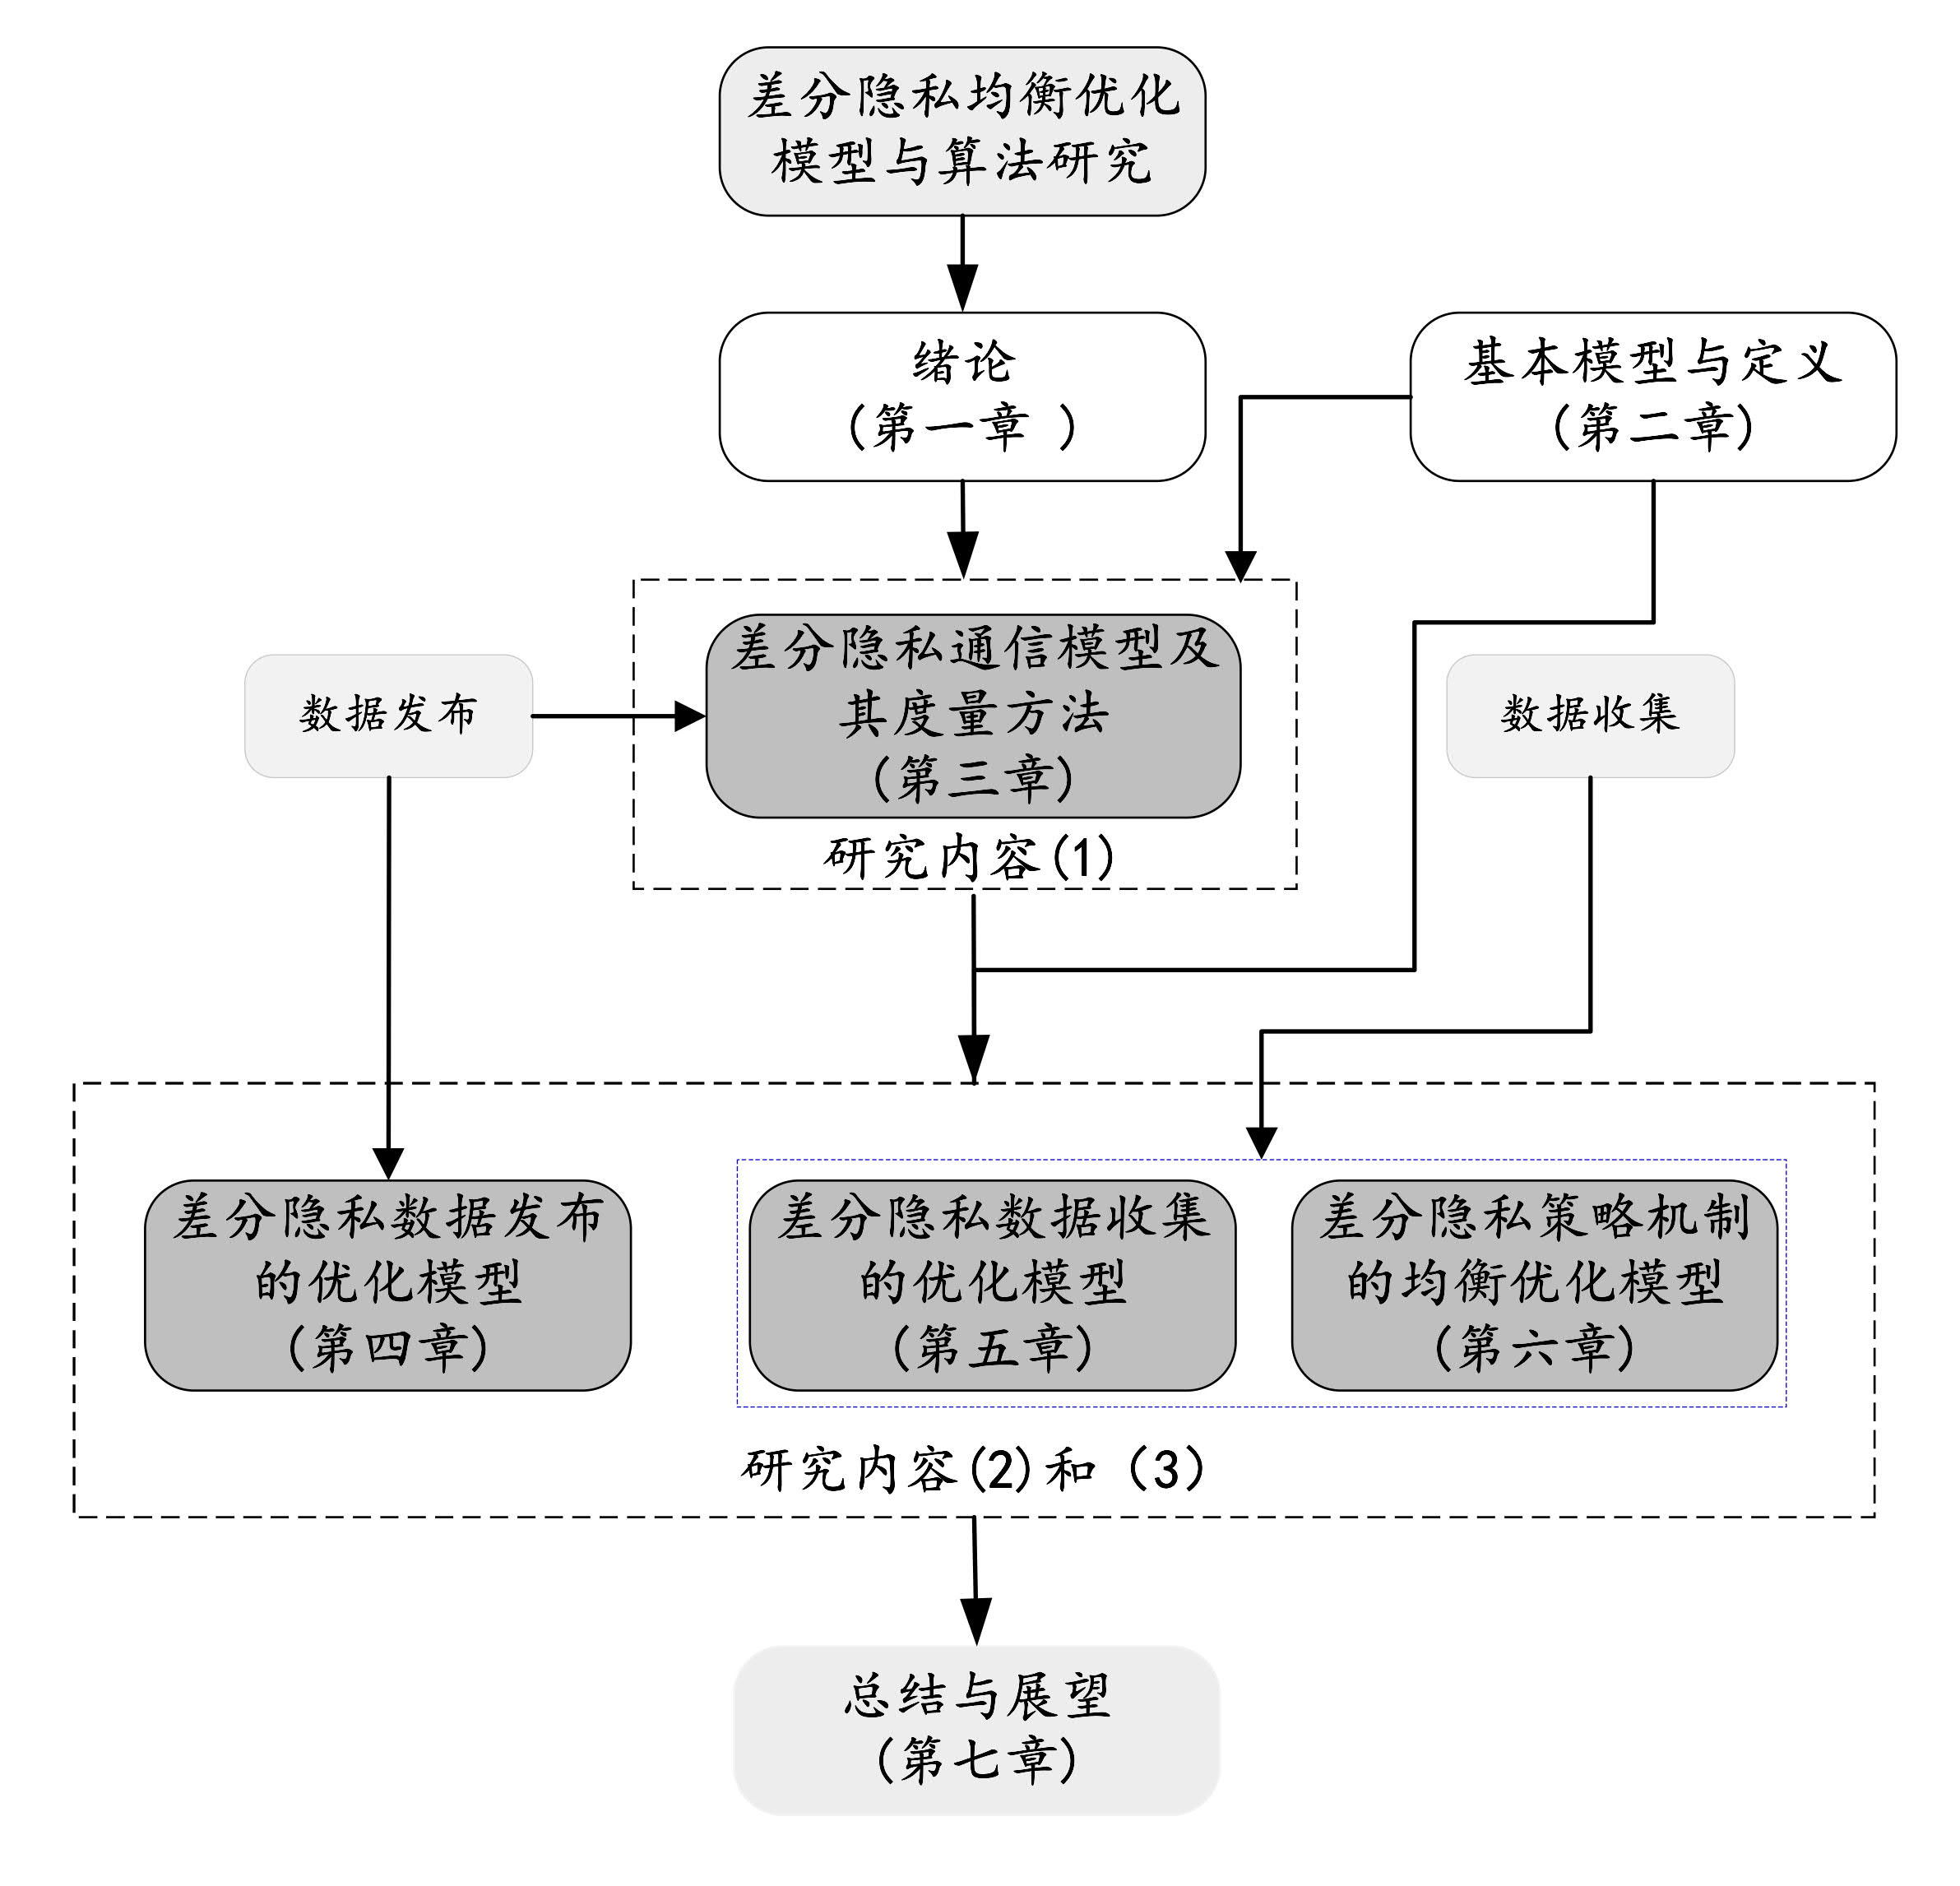
\includegraphics[width = 0.7\linewidth]{./figures/chapter01_2.jpg}
	\caption{本文的章节内容组织结构图}
	\label{fig:chapter1-research-structure}
\end{figure}

第\ref{chapter01}章为\textit{绪论},首先阐述了本文的研究背景及意义,随后针对差分隐私分析了存在的问题,凝练出本文研究需要解决的关键问题。基于上述分析,阐述了本文的研究内容和研究取得的主要成果。最后给出了本文的章节组织结构安排。



第\ref{chapter02}章为{\em 基本模型与定义},介绍了本文研究所使用的基本模型与定义。首先,给出了隐私、隐私泄露的定义,并阐述了差分隐私模型及定义。其次,叙述了Shannon信息论的通信模型,引入信息熵、条件熵、联合熵、互信息量等概念,以此为基础介绍了数据处理不等式、费诺不等式和率失真理论等内容。随后,阐述了最优化问题、对策博弈以及凹凸博弈的相关知识。最后,以上述为基础,给出了本文中差分隐私均衡优化的定义,界定后续研究的范畴。


第\ref{chapter03}章为{\em 差分隐私通信模型及其度量方法},建立差分隐私与信息论的基本联系,奠定本文的研究基础。首先,基于Shannon基本通信模型,介绍了差分隐私基本通信模型,并给出了形式化的模型表达。其次,以差分隐私的基本通信模型为基础,引入信息熵、互信息、失真的概念对隐私与效用进行度量,提出信息熵度量模型及方法。进一步,在基本的度量基础上,针对多维关联属性的情景,提出面向关联属性的差分隐私信息熵度量方法,本章中的度量模型及方法为开展后续章节的研究奠定了基础。

第\ref{chapter04}章为{\em 差分隐私数据发布的优化模型},研究了隐私与数据效用权衡的最优差分隐私机制。首先,基于第\ref{chapter02}章基础、第\ref{chapter03}章差分隐私通信模型及度量方法,分析了隐私系统的目标,借鉴率失真理论构建了面向差分隐私数据发布的优化模型。其次,在基本的通信模型基础上引入敌手模型,并考虑了敌手拥有关联辅助背景知识对隐私泄露的影响,提出了基于联合事件的互信息隐私度量。随后,修改率失真表述形式,提出了最小化隐私泄露的优化模型,用于获得隐私机制的概率分布函数。此外,设计了互信息隐私最优信道机制的近似迭代求解算法,并给出具体的验证分析。

第\ref{chapter05}章为{\em 差分隐私数据收集的优化模型},围绕隐私保护机制设计的两个阶段,研究了面向数据收集的多维数据最优隐私机制。首先,以第\ref{chapter03}章的度量为基础,形式化互信息隐私(MI-privacy)最优化模型,设计模型求解算法寻找最优机制的概率密度函数。随后,将其作为基本构建模块应用到多维数据,提出有序随机响应扰动(ORRP)方案。最后,针对提出的ORRP方案,介绍了隐私、数据效用以及相关度损失的评估与分析,并利用真实数据集给出了所提方案的实验分析。


第\ref{chapter06}章为{\em 差分隐私策略机制的均衡优化模型},应用博弈均衡理论研究了差分隐私策略机制选择问题。通过分析隐私保护系统参与者的隐私目标,基于信息熵度量模型及方法将隐私目标形式化为隐私泄露的极大极小问题。然后,分析系统参与者的可行策略,构建了隐私保护的攻防博弈(PPAD)模型。针对本文关注的应用,实例化PPAD为两方零和对策博弈模型,并提供了均衡的理论分析以及算法实现。最后,阐述了均衡在隐私保护中的内涵及意义。


第\ref{chapter07}章为\textit{总结与展望},首先总结了本文的研究工作,进一步,展望了未来研究工作的方向和重点。


